% Separate IFG supplementary: descriptive development evidence only.
\documentclass[10pt,twocolumn,letterpaper]{article}
\usepackage[T1]{fontenc}
\usepackage[review]{cvpr}
% Project additions; no margin, font-size, or spacing overrides.
\usepackage{amsmath,amssymb}
\usepackage{booktabs}
\usepackage{tabularx}
\usepackage{xcolor}
\usepackage{tikz}
\usetikzlibrary{positioning,arrows.meta,fit,calc,backgrounds}
\usepackage{algorithm}
\usepackage{algpseudocode}
\newif\ifhasverifiedreferences
\hasverifiedreferencestrue % Draft 1: 19 entries; each copied from a local PDF or a publisher page.
\newcommand{\draftnote}[1]{\par\noindent\textbf{Draft status:} #1\par}
\newcommand{\notmeasured}{\textit{n/m}}
% Pending content is shown in red and must be resolved or removed before submission.
\newcommand{\tbd}[1]{{\color{red}[TBD: #1]}}
% Numbers traceable to a verify.json / summary.json but not yet in paper/evidence registry: dark orange in draft.
% Redefine as identity (\renewcommand{\pend}[1]{#1}) once the registry audit passes.
\newcommand{\pend}[1]{{\color{orange!75!black}#1}}
\newcommand{\sys}{AG3S}% method name as in the working title
\newcommand{\dmain}{d}
\newcommand{\dfree}{d^{\star}}

\definecolor{cvprblue}{rgb}{0.21,0.49,0.74}
\usepackage[pagebackref,breaklinks,colorlinks,allcolors=cvprblue]{hyperref}
% Working metadata, separate from the immutable official kit.
\def\paperID{*****} % Replace with the actual registered OpenReview paper ID.
\def\confName{CVPR}
\def\confYear{2027} % Local target year; does NOT make this a 2027 official kit.
\title{AG3S VLA: Grounding VLA Attention in 3D\\for Task-Dependent Contact Constraints}% revised working title; subject to final results
\author{Anonymous Authors}

\begin{document}
\maketitlesupplementary
\section{Frozen parameters}
\begin{table}[h]
\centering
\caption{\textbf{Parameters fixed on development data} and frozen before every held-out and closed-loop evaluation.}
\label{tab:supp-params}
\small
\begin{tabular}{ll}
\toprule
Voxel size & 5\,mm\\
Robot-depth tolerance $\epsilon_r$ & 10\,mm\\
Depth-edge / node-distance thresholds & 10\,mm / 15\,mm\\
Affinity $\sigma_x$, $\sigma_n$ & 10\,mm, 0.2\\
Seed neighborhood & 15\,cm\\
Noun attention head & prefix layer 10, head 7\\
Seed patches / eligibility & top 5 / $\geq$ 60 non-robot, non-support pixels\\
Membership threshold & 0.5\\
Identity features & prefix layer 8, centered\\
Candidate components & $\geq$ 20 nodes, bounding box $\leq$ 0.4\,m\\
Switch margin $\kappa$ / alert threshold & 0.05 / 0.59\\
Probe features & layer-4 key/value, pooled\\
Chunk $H$ / refined $J$ / executed $K$ & 50 / 16 / 8\\
TSDF voxel (cuRobo) & 5\,mm\\
ESDF coarse grid / fine hand window & 20\,mm / 5\,mm, query = minimum of the two\\
Unobserved space in the scene field & free\\
\bottomrule
\end{tabular}
\end{table}

\section{One episode, moment by moment}
\begin{figure*}[h]
\centering
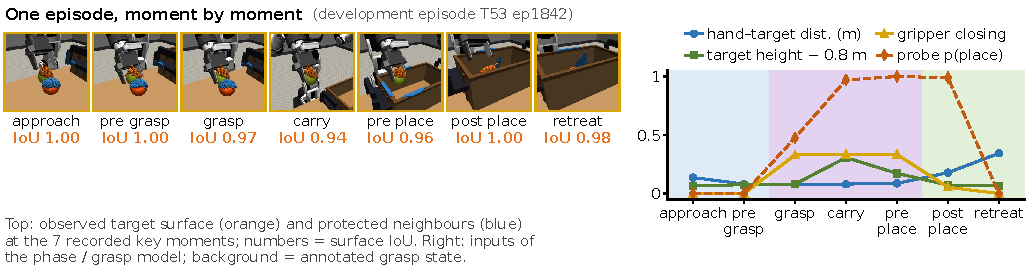
\includegraphics[width=\textwidth]{../figures/cvpr_v1/fig06_episode_strip.pdf}
\caption{\textbf{A development episode at seven key moments.} \emph{Top:} the observed target surface (orange) and protected neighbors (blue), with the surface IoU of each moment. \emph{Bottom:} inputs of the phase and grasp model over the same moments.}
\label{fig:supp-episode}
\end{figure*}

\section{Diagnostic reruns of the held-out closed-loop failures}
On the 34 held-out seeds selected because the coarse configuration had succeeded, our configuration failed six. Each was rerun with the extent and the robot mask varied independently (Tab.~\ref{tab:supp-diag}). Substituting the simulator's visible target surface rescues two seeds regardless of the mask; the sphere mask with our surface rescues two different seeds; the mechanism behind the remaining failures is not isolated. In the failed runs the selected region also removed basket samples (159--431 per chunk in five of six), a correlate of identity drift rather than an established cause.
\begin{table}[h]
\centering
\caption{\textbf{Failure reruns (outcome per seed).} Coarse = radius growth + ball exemption; ours = surface + rendered mask; GT = simulator-visible target surface; ``sphere'' = sphere/capsule robot filter.}
\label{tab:supp-diag}
\footnotesize
\setlength{\tabcolsep}{3.5pt}
\begin{tabular}{lcccccc}
\toprule
Seed & Coarse & Ours & Ours (rerun) & GT + render & Ours + sphere & GT + sphere\\
\midrule
391 & ok & no grasp & no grasp & ok & no grasp & ok\\
764 & ok & no grasp & no grasp & no grasp & no grasp & no grasp\\
1769 & ok & no grasp & no grasp & ok & regrasp, failed & ok\\
623 & ok & no grasp & no grasp & no grasp & no grasp & no grasp\\
1893 & ok & no grasp & no grasp & slip at lift & ok & slip at lift\\
485 & ok & not placed & not placed & slip at lift & ok & slip at lift\\
\bottomrule
\end{tabular}
\end{table}

\section{Development ablation tables}
The following tables report the development-set component comparisons (180 selected frames, 32 episodes, replayed depth) that the main paper summarizes in prose. All settings were later frozen before the held-out evaluation in the main paper.

\begin{table}[h]
\centering
\caption{\textbf{Matched-mask surface grounding (development).} Episode-mean metrics. ``Volume'' and ``render'' denote robot removal. Empty predictions contribute zero IoU/recall; undefined precision is omitted for 5/1/3/1/3/1 frames in row order.}
\label{tab:supp-extent}
\small
\begin{tabular}{llccc}
\toprule
Extent & Mask & IoU & Prec. & Recall\\
\midrule
Radius + clustering & Volume & .785 & .896 & .828\\
Surface graph & Volume & .817 & .947 & .831\\
Radius + clustering & Render & .837 & .865 & .910\\
Surface graph & Render & .893 & .938 & .915\\
Enclosing ball & Render & .778 & .809 & .903\\
Surface + reassociation & Render & .912 & .957 & .933\\
\bottomrule
\end{tabular}
\end{table}

\begin{table}[h]
\centering
\caption{\textbf{Feature fusion with the improved geometry fixed (development).} Episode-mean IoU, rendered robot mask, largest-seed-mass region selection. Prefix layer 8 is shown; projector and prefix layers 4 and 12 behave alike. Oracle seeds are diagnostic inputs, not a deployable method.}
\label{tab:supp-features}
\small
\begin{tabular}{lc}
\toprule
Membership construction & IoU\\
\midrule
Geometry + attention seeds & .893\\
+ Feature edges & .893\\
+ Prototype unary & .827\\
+ Feature edges and unary & .826\\
Feature-conditioned region growing & .755\\
Geometry region growing & .832\\
Edges + unary, shuffled features & .485\\
Geometry, oracle target seeds & .918\\
\bottomrule
\end{tabular}
\end{table}

\begin{table}[h]
\centering
\caption{\textbf{Auxiliary phase prediction (development).} Pooled accuracy over 180 selected frames; LR denotes logistic regression with leave-one-episode-out fitting. Upstream grounding and feature choices are shared across folds.}
\label{tab:supp-phase}
\small
\begin{tabular}{lc}
\toprule
Phase predictor & Accuracy\\
\midrule
HSR argmax & .783\\
LR: HSR & .856\\
LR: HSR + gripper & .878\\
LR: HSR + gripper + geometry & .939\\
+ Memory agreement & .933\\
\bottomrule
\end{tabular}
\end{table}

\section{Development experiment gallery}
This supplement documents the component experiments behind configuration B: attention-seeded surface extent, centered-feature identity switching, confidence alerts, and geometric task-state inference. All examples come from the same 180 selected frames / 32 development episodes as the main paper. No new held-out or closed-loop result is introduced.

The gallery follows the experimental questions rather than presenting selected images as average performance. Selection rules are stated in each caption; several examples deliberately maximize a gain or loss. Ground-truth colors diagnose predictions and are not algorithm inputs. Green/orange/blue typically denote true positives/false positives/false negatives; the confidence figure uses region identity labels and the centering figure uses cosine color scales.

The adopted switch has a development gain of $+0.019$ with interval $[-0.020,0.060]$. Its adoption is a design choice pending validation, not a positive test result. The no-switching configuration A is the matched ablation. The alert and phase experiments below use the base surface selection, so their results do not establish the performance of the combined B configuration.

The phase height input is centroid $z$ minus a floor-dominated support median, effectively base-frame height. Calling it height above the table is incorrect. The fixed-height scenes do not establish robustness to support-height variation.
\begin{figure*}[p]
\centering
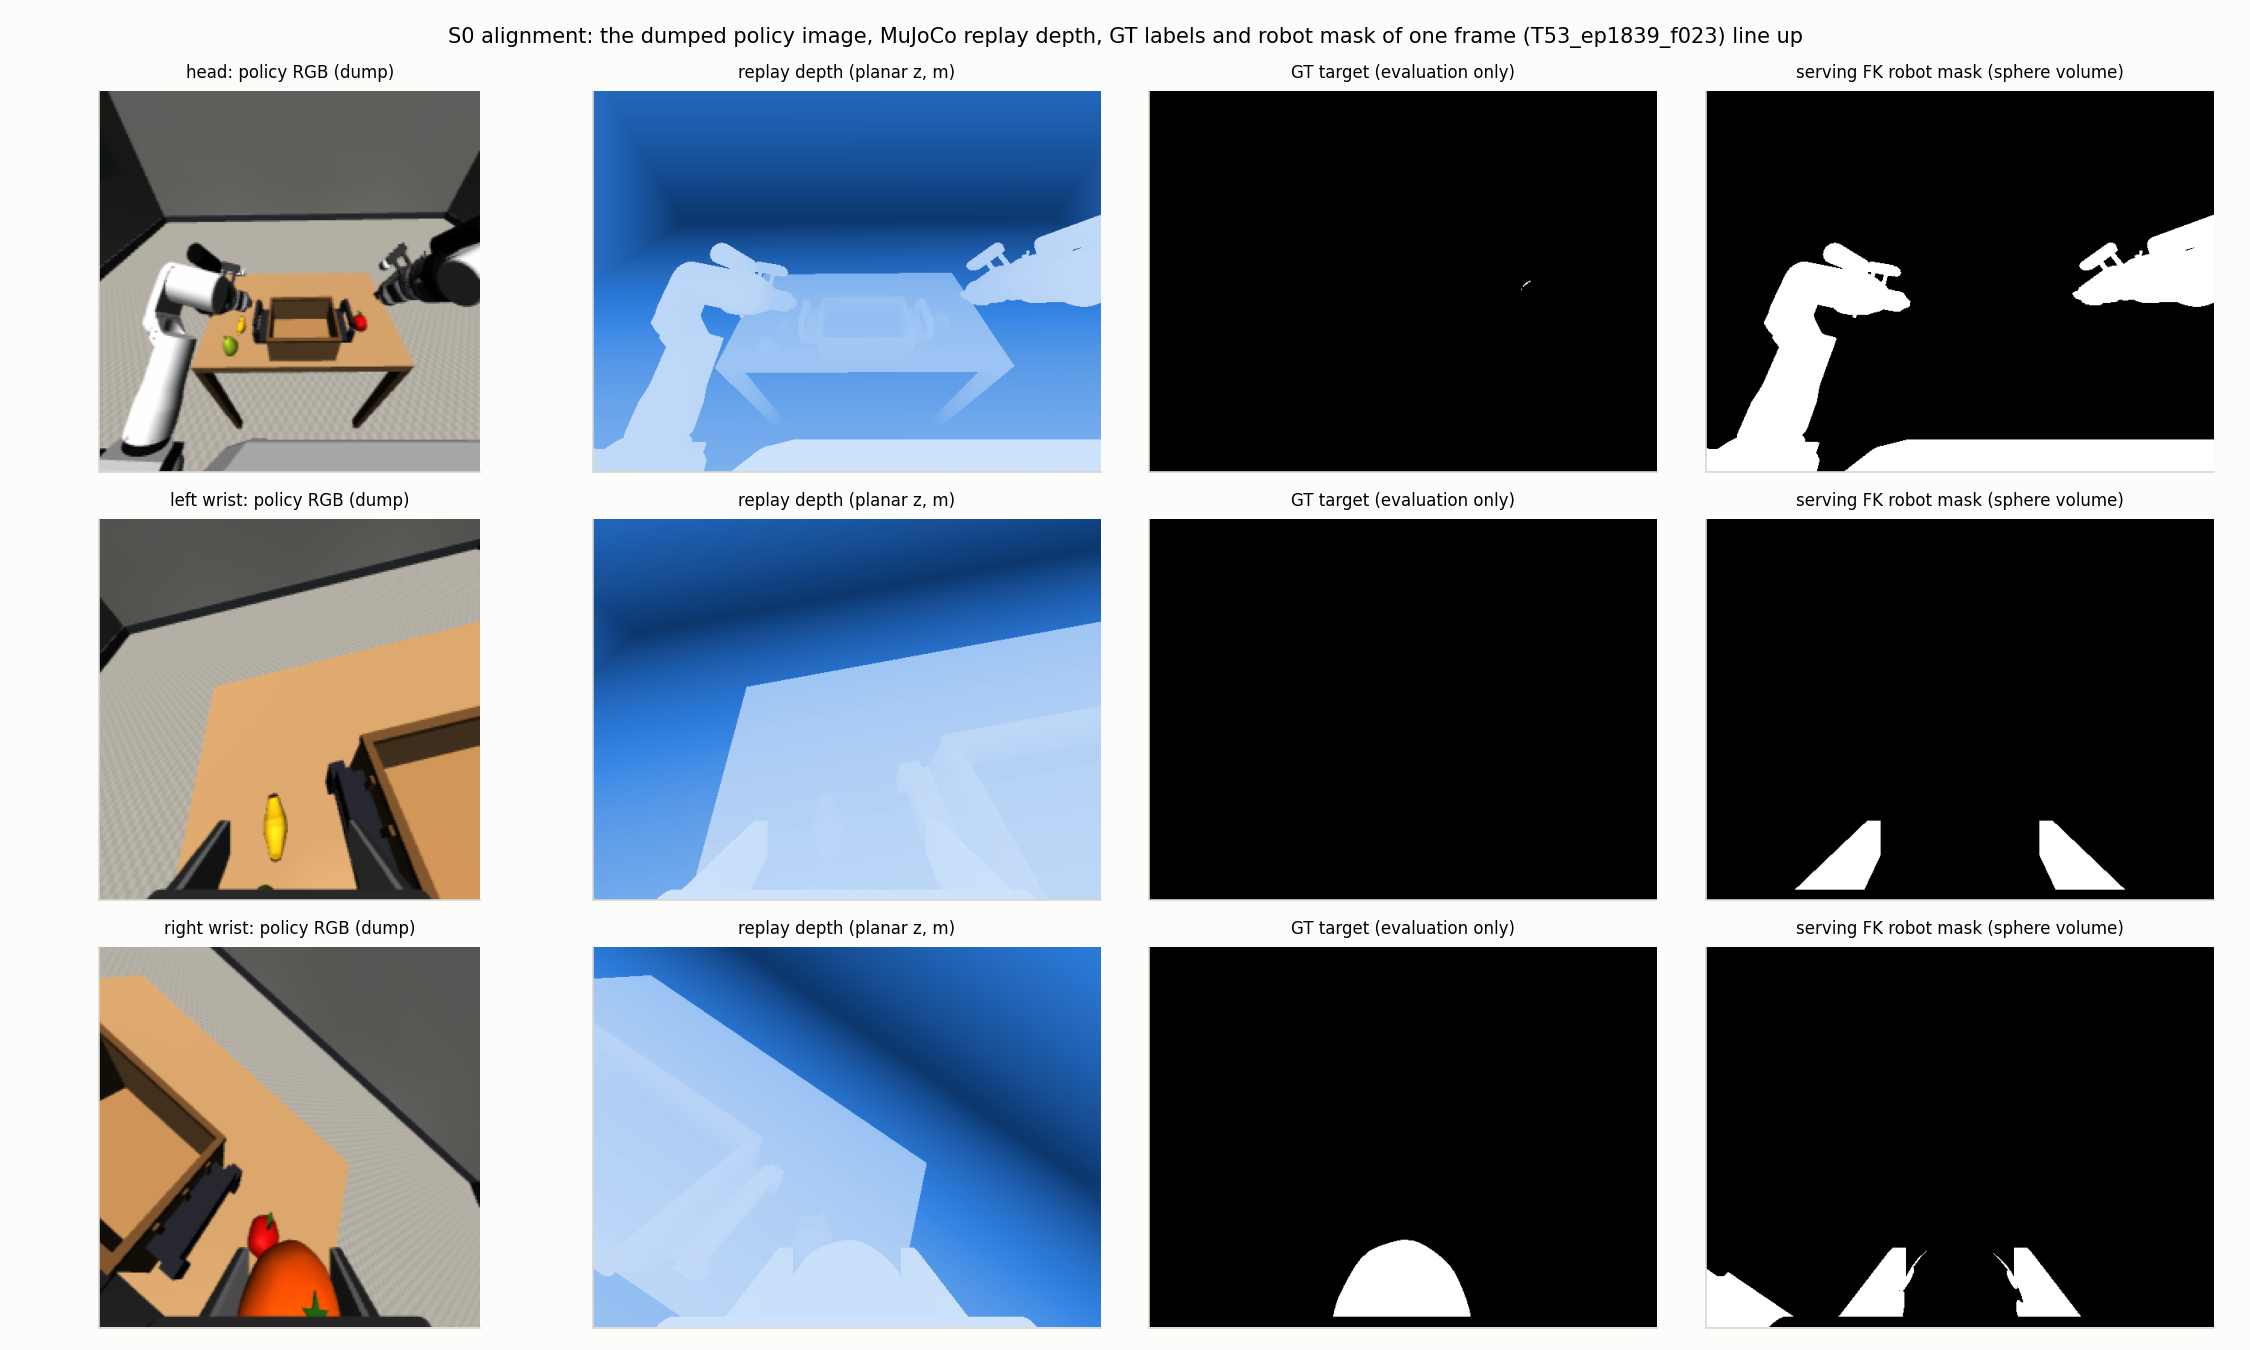
\includegraphics[width=\textwidth,height=.70\textheight,keepaspectratio]{../figures/ifg_results/exp/exp-S0-alignment.png}
\caption{\textbf{S0: alignment.} Do image, attention, depth, and evaluation labels refer to the same scene? All 180 frames passed the recorded alignment checks after documented preprocessing corrections. This example comes from the protocol debug-frame family; it is not a segmentation comparison.}
\label{fig:supp-exp-S0-alignment}
\end{figure*}

\begin{figure*}[p]
\centering
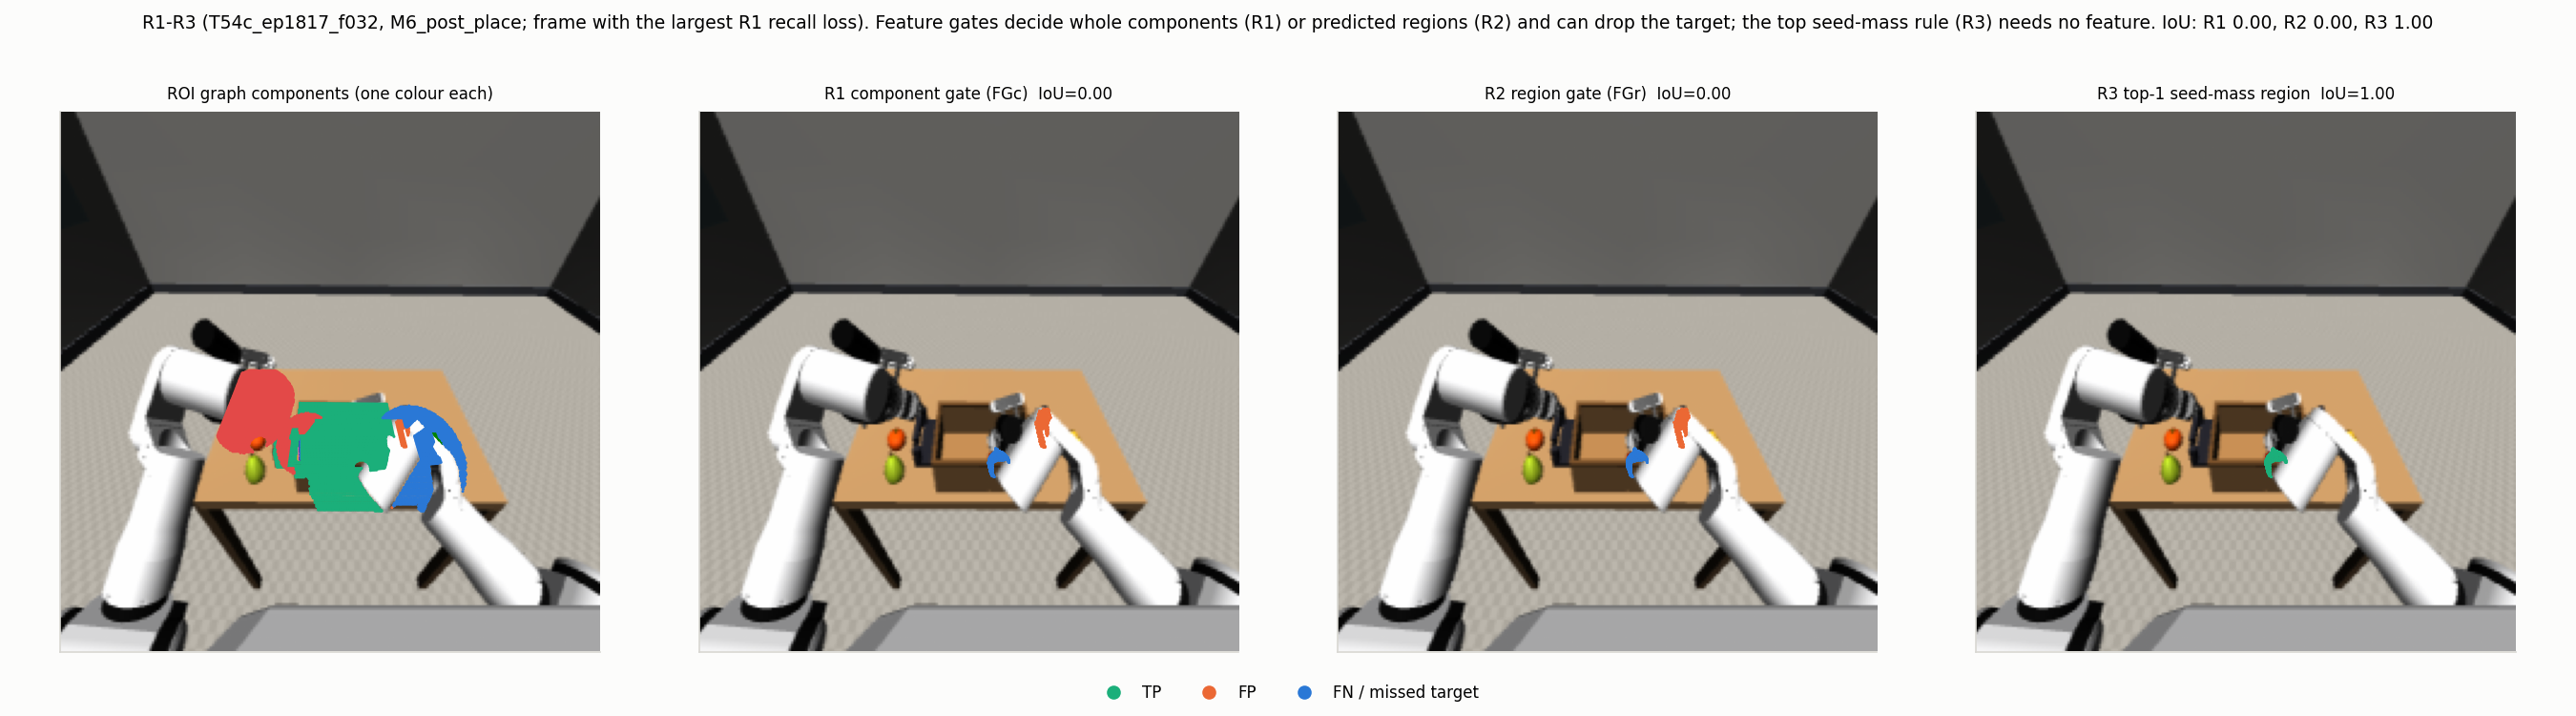
\includegraphics[width=\textwidth,height=.70\textheight,keepaspectratio]{../figures/ifg_results/exp/exp-R1-R3-gate-unit.png}
\caption{\textbf{R1--R3: the unit of feature gating.} Can feature gates rescue boundary estimation? Component-level and region-level gates can discard the target. This frame maximizes the recall loss of the first component gate relative to geometry-only membership. Later top-region selection helped even without features, motivating the seed-mass selection rule.}
\label{fig:supp-exp-R1-R3-gate-unit}
\end{figure*}

\begin{figure*}[p]
\centering
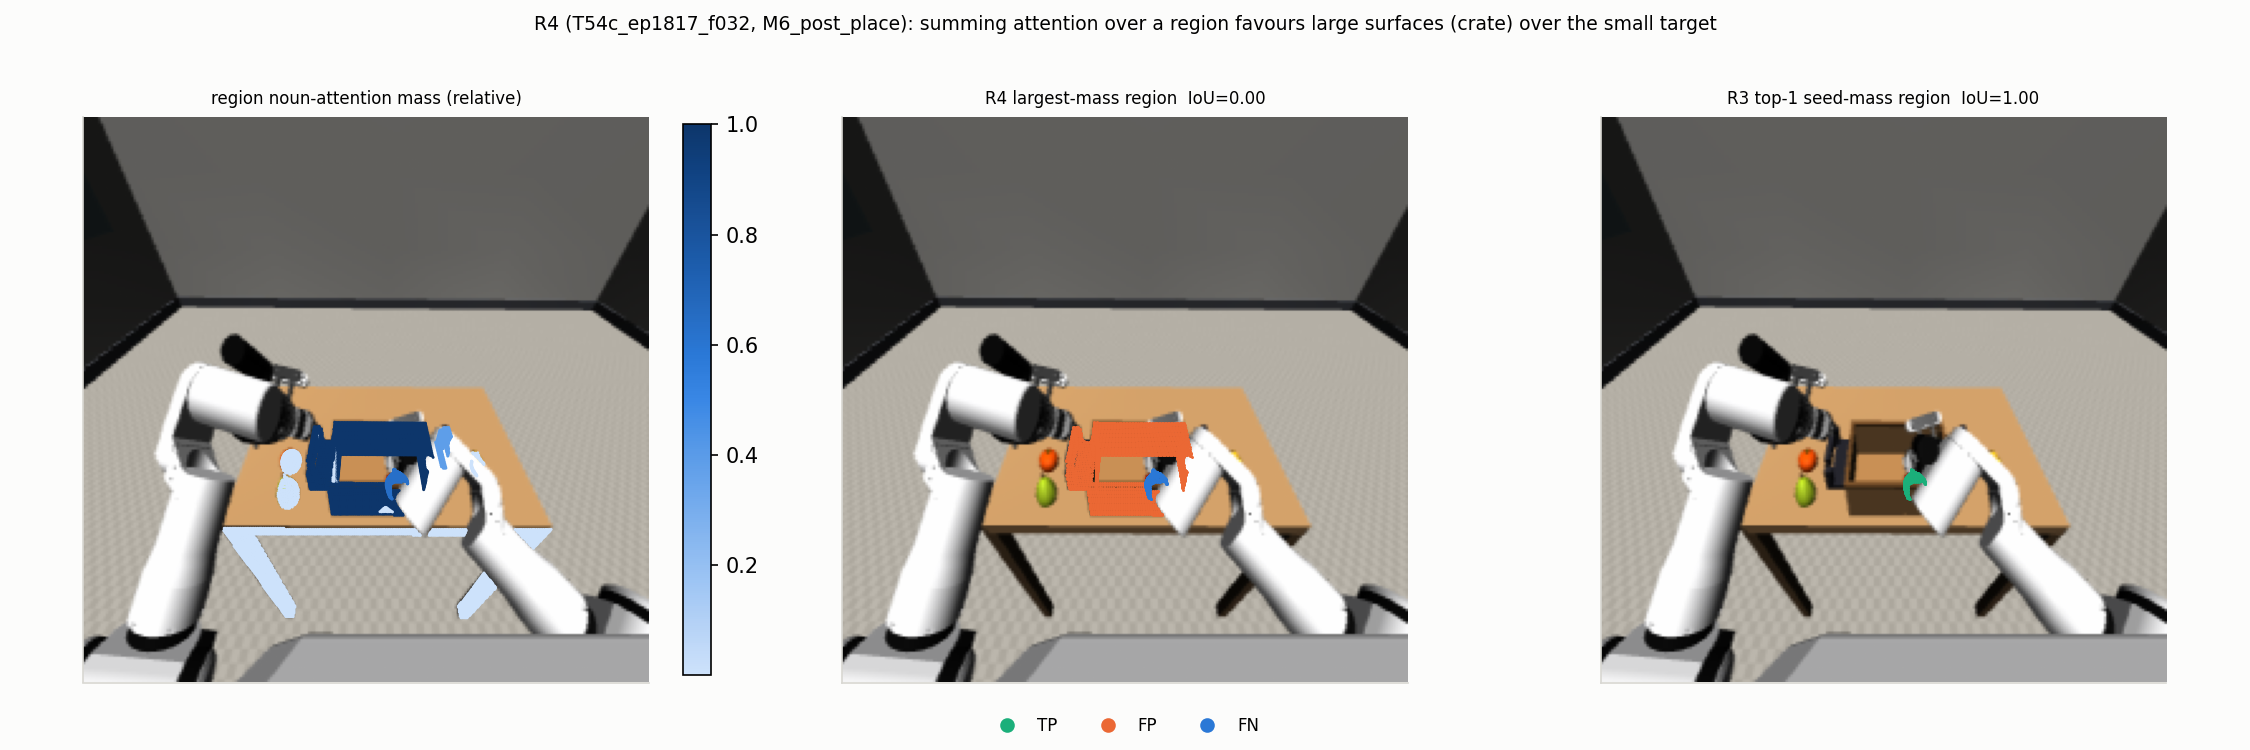
\includegraphics[width=\textwidth,height=.70\textheight,keepaspectratio]{../figures/ifg_results/exp/exp-R4-mass-bias.png}
\caption{\textbf{R4: attention-mass size bias.} Does ranking whole regions by total attention help? The displayed frame maximizes the IoU loss of total-mass ranking relative to the top-seed-mass rule. A large destination can win by size. The oracle region-selection diagnostic (0.843 IoU) is conditional on this older candidate set, not a full ground-truth-mask baseline or a universal upper bound.}
\label{fig:supp-exp-R4-mass-bias}
\end{figure*}

\begin{figure*}[p]
\centering
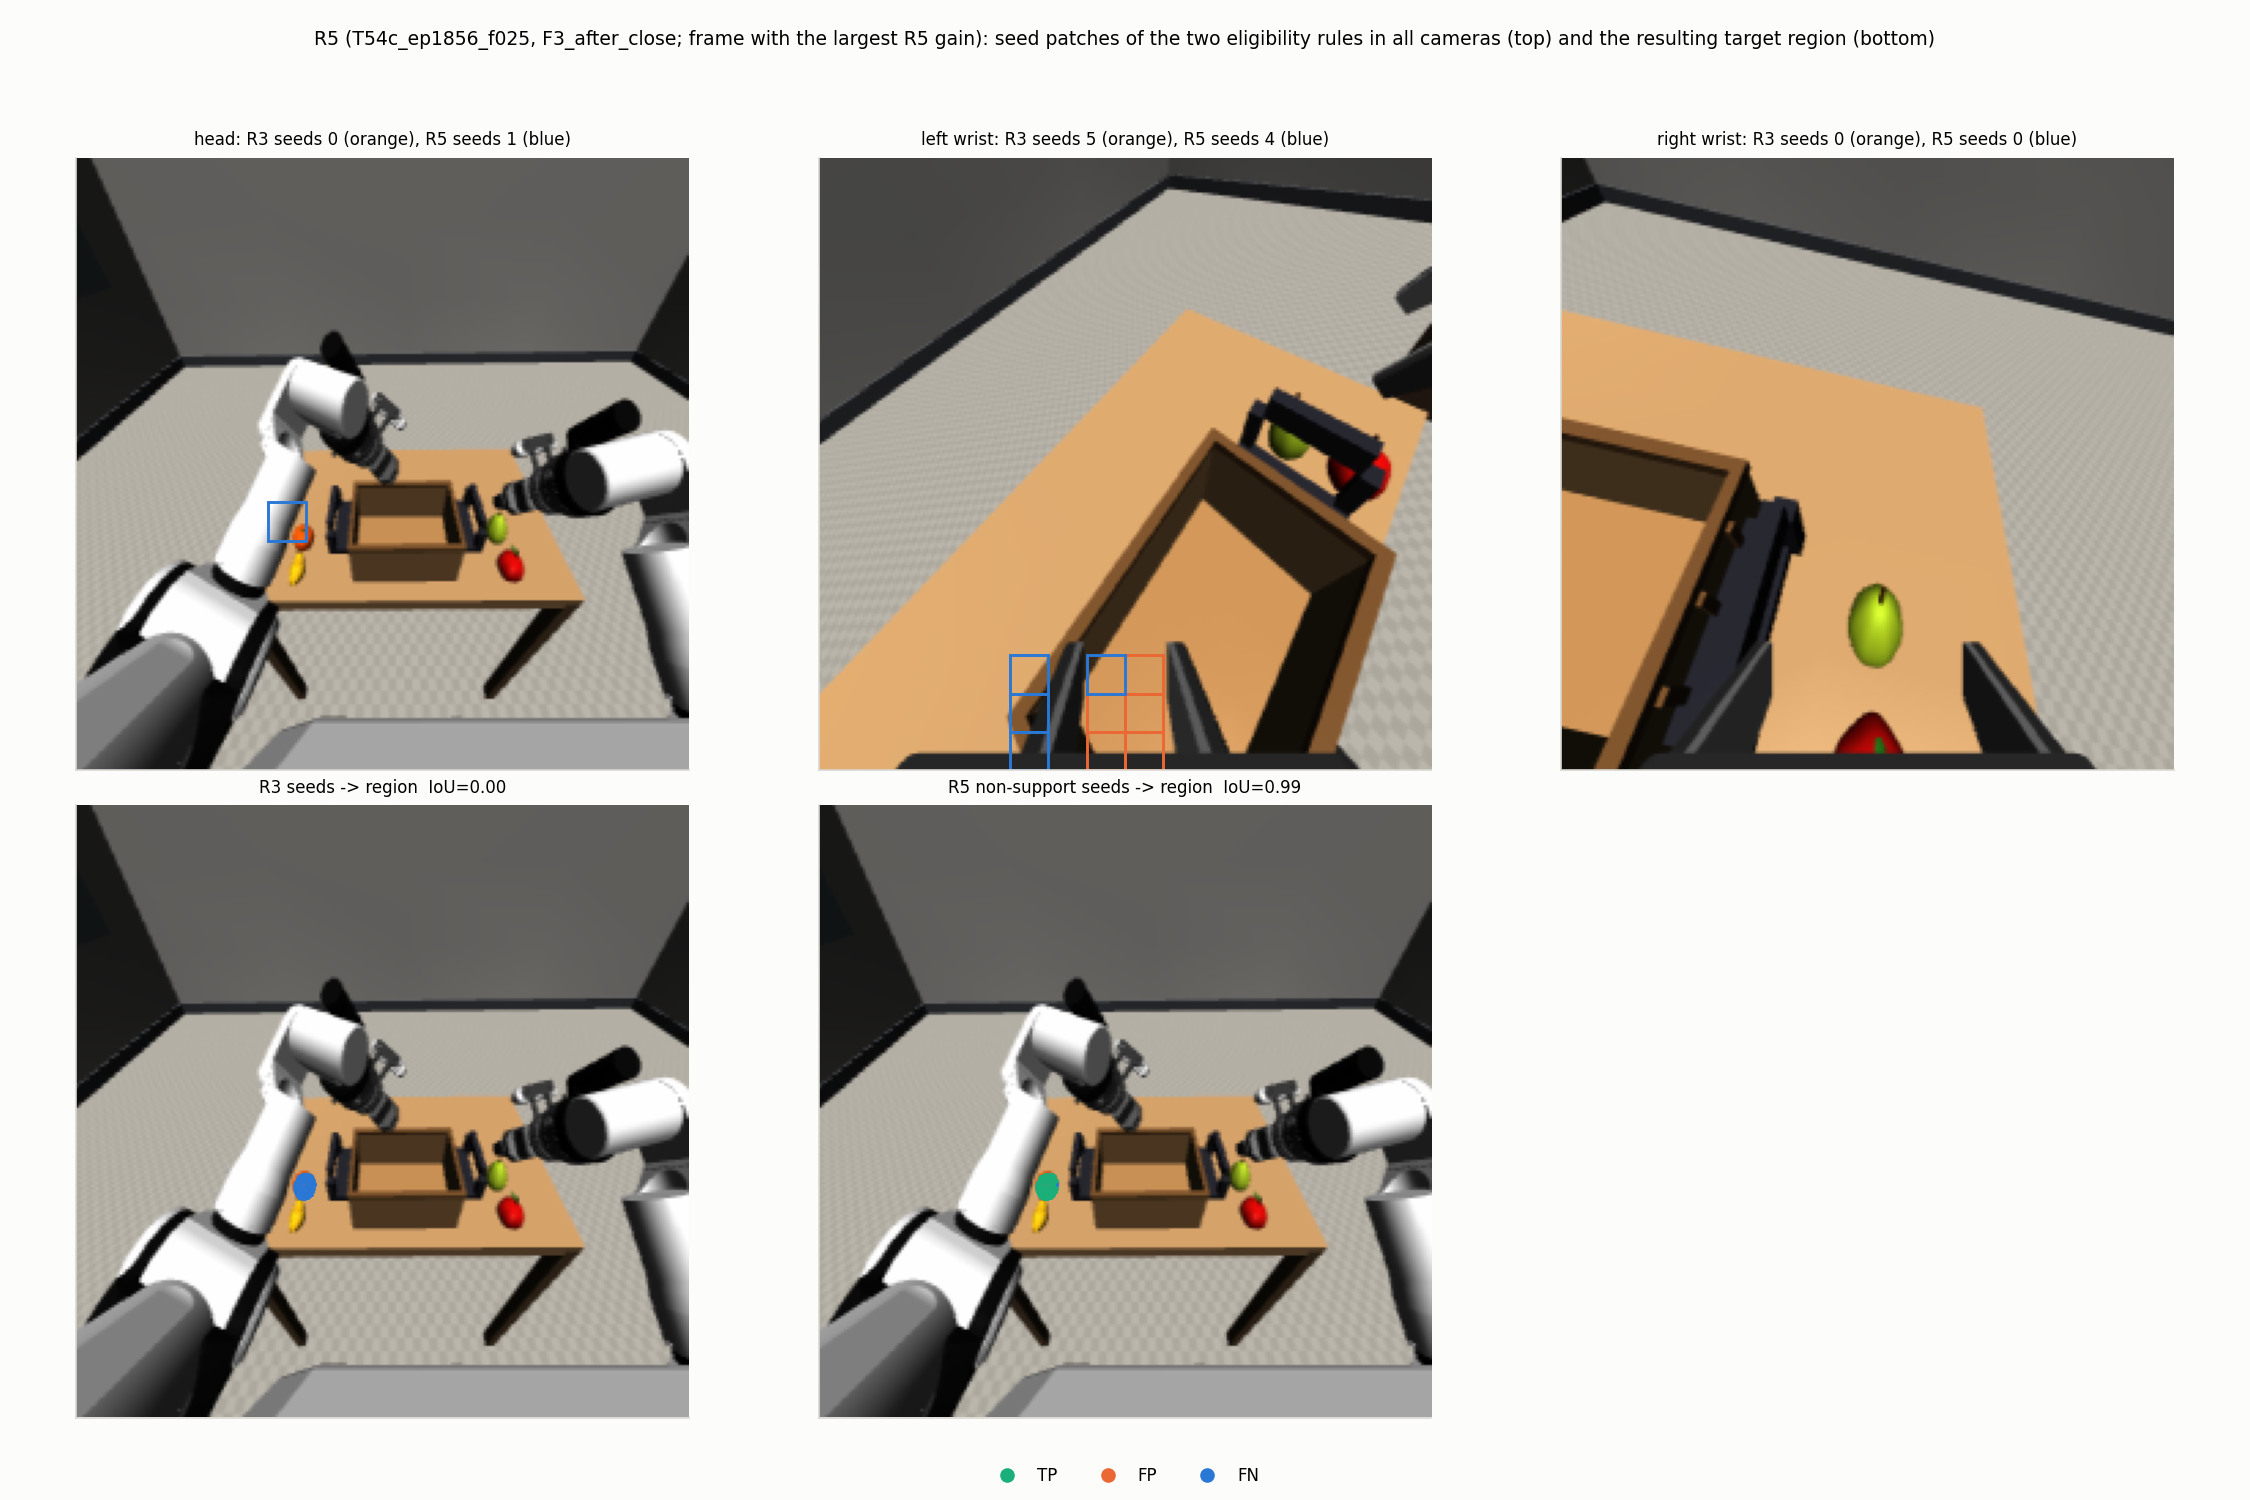
\includegraphics[width=\textwidth,height=.70\textheight,keepaspectratio]{../figures/ifg_results/exp/exp-R5-nonsupport-seed.png}
\caption{\textbf{R5: seed eligibility.} Does excluding support-dominated seed candidates help? The example maximizes the IoU gain from the non-support eligibility rule and shows all three cameras. The rule requires at least 60 non-robot, non-support pixels; it does not remove every support pixel from a selected patch. Aggregate IoU improves from 0.794 to 0.817 on development data.}
\label{fig:supp-exp-R5-nonsupport-seed}
\end{figure*}

\begin{figure*}[p]
\centering
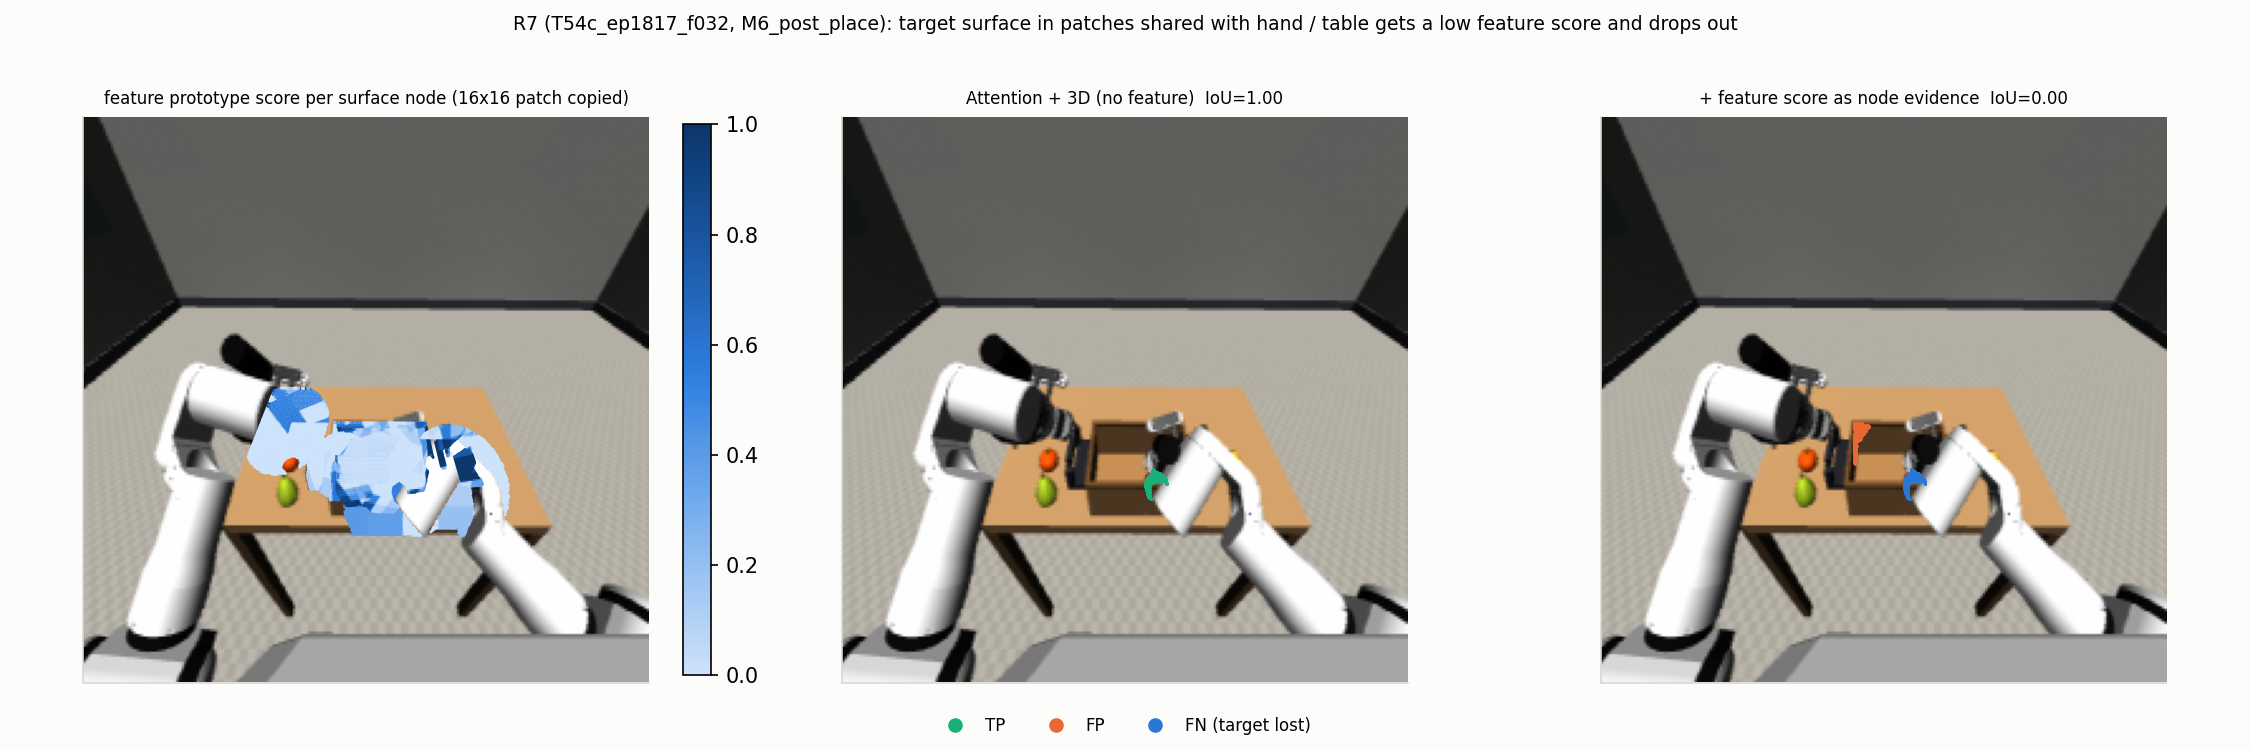
\includegraphics[width=\textwidth,height=.70\textheight,keepaspectratio]{../figures/ifg_results/exp/exp-R7-feature-unary-loss.png}
\caption{\textbf{R7: prototype-unary loss.} Does feature fusion help after correcting seeds and robot masking? This frame maximizes the IoU loss from a prefix-layer-8 prototype unary relative to the improved geometric parent. The ablation therefore exposes a failure under the stronger geometry setting, rather than attributing early preprocessing failures to features.}
\label{fig:supp-exp-R7-feature-unary-loss}
\end{figure*}

\begin{figure*}[p]
\centering
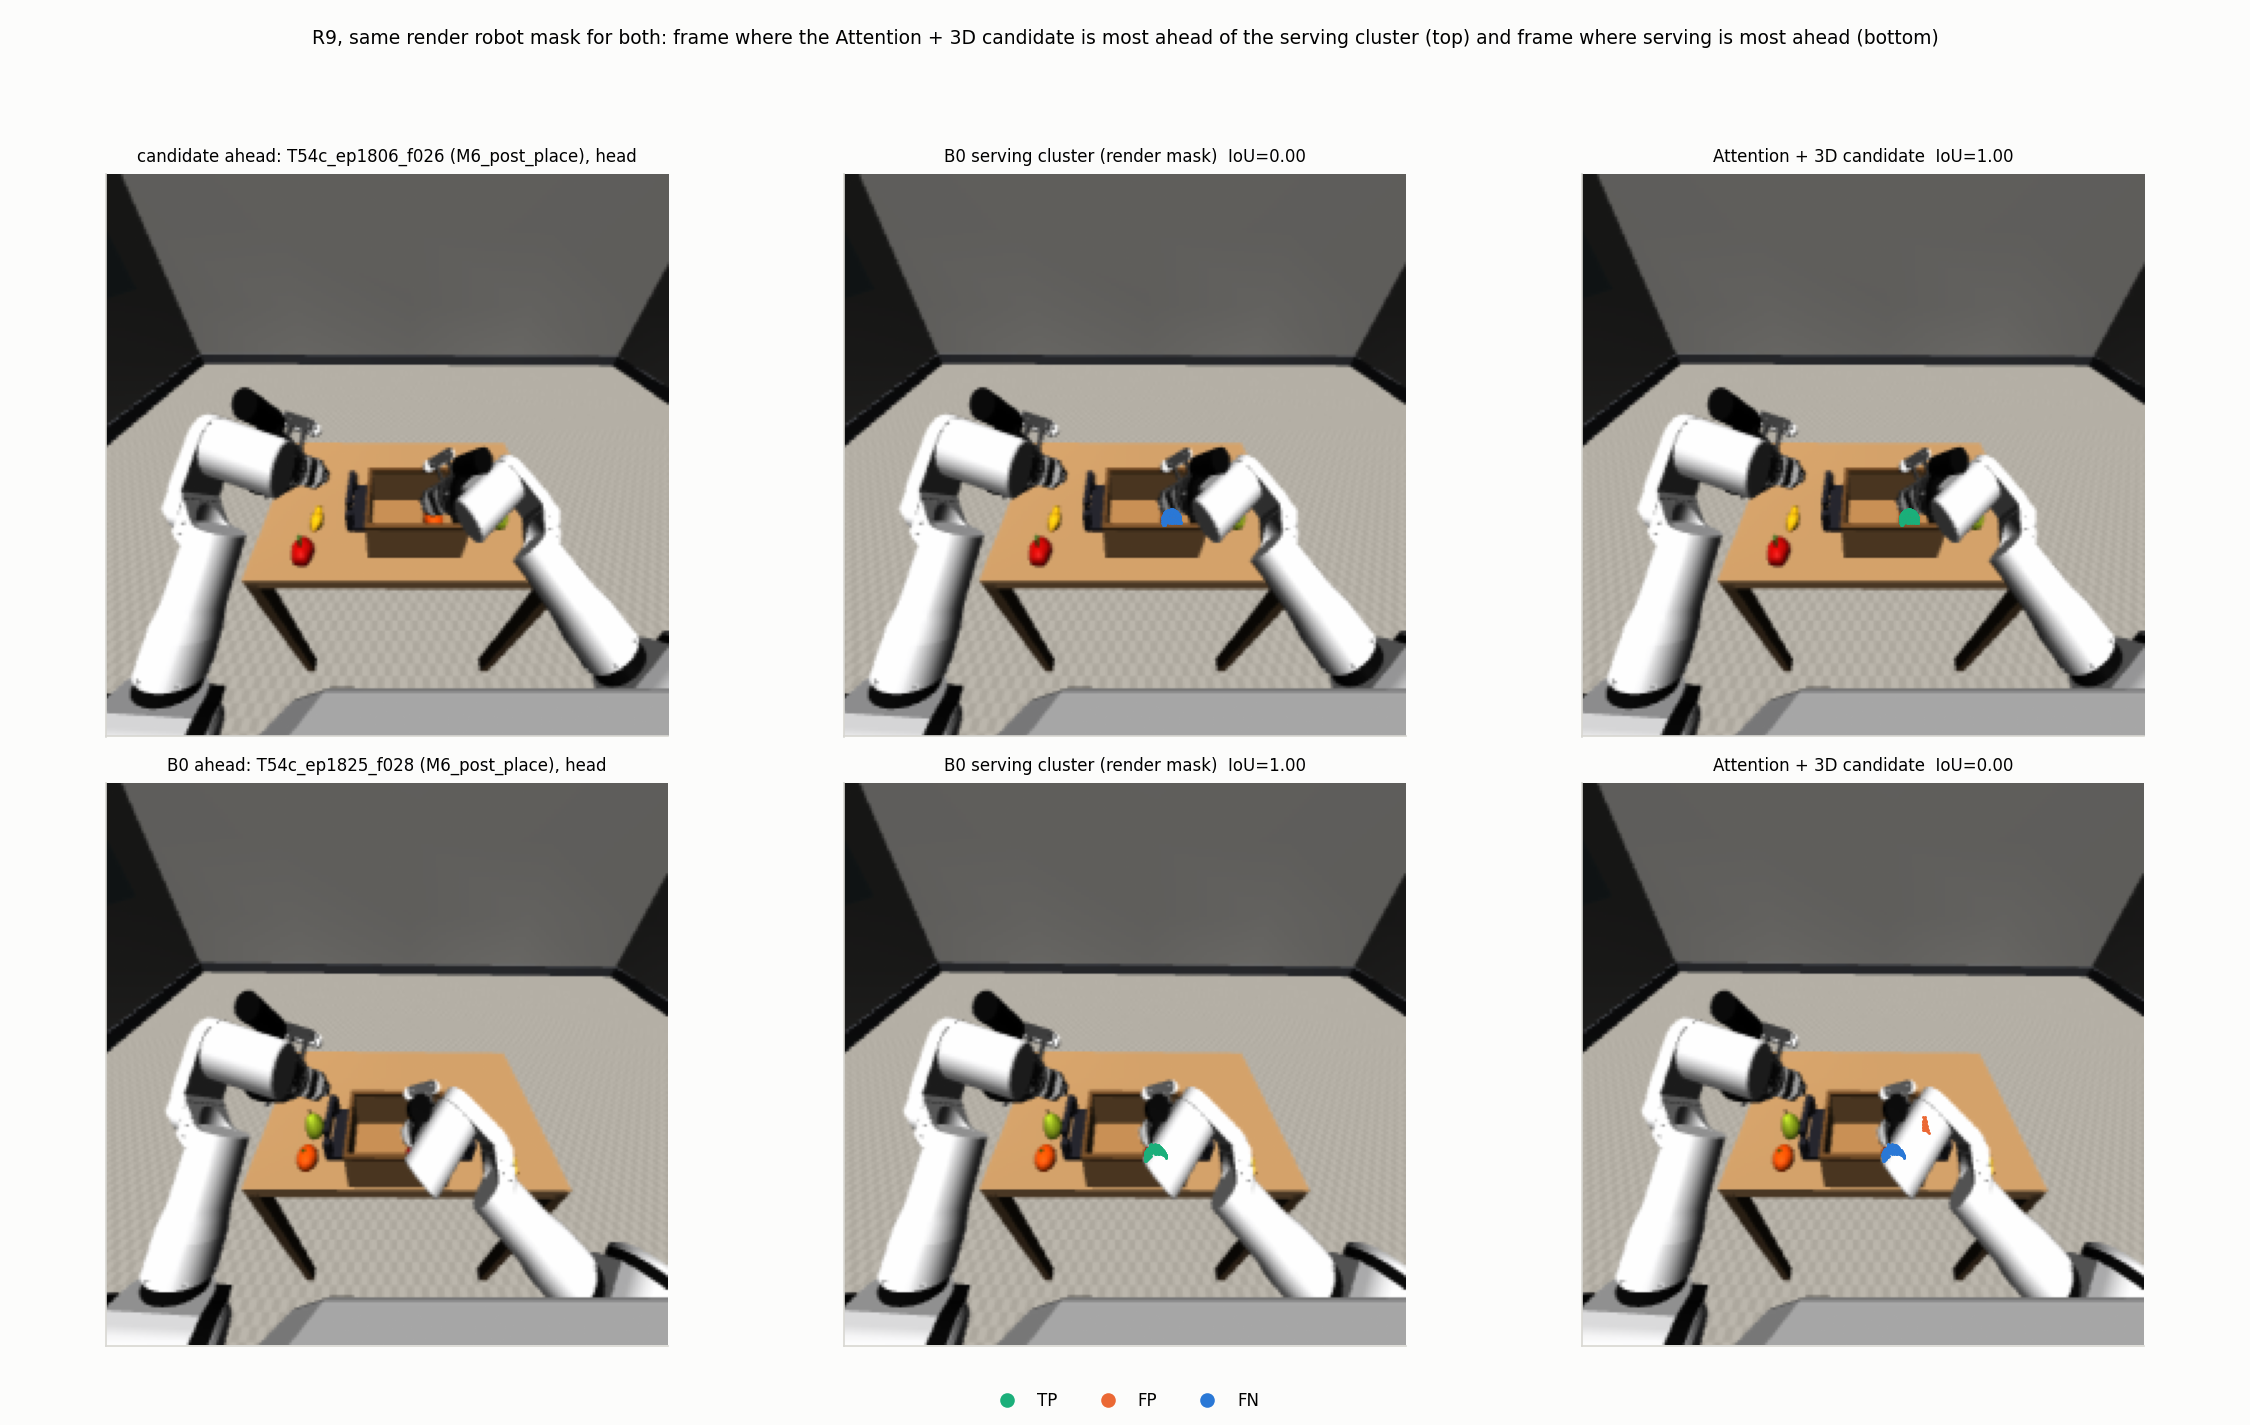
\includegraphics[width=\textwidth,height=.70\textheight,keepaspectratio]{../figures/ifg_results/exp/exp-R9-vs-serving.png}
\caption{\textbf{R9: matched-mask successes and failures.} Which frames favor each extent method when both receive the rendered robot mask? The top and bottom examples maximize and minimize the candidate-minus-baseline IoU difference. Both are post-placement examples. Their extremes, 1 versus 0 and 0 versus 1, are selected illustrations; aggregate development IoU is 0.893 versus 0.837.}
\label{fig:supp-exp-R9-vs-serving}
\end{figure*}

\begin{figure*}[p]
\centering
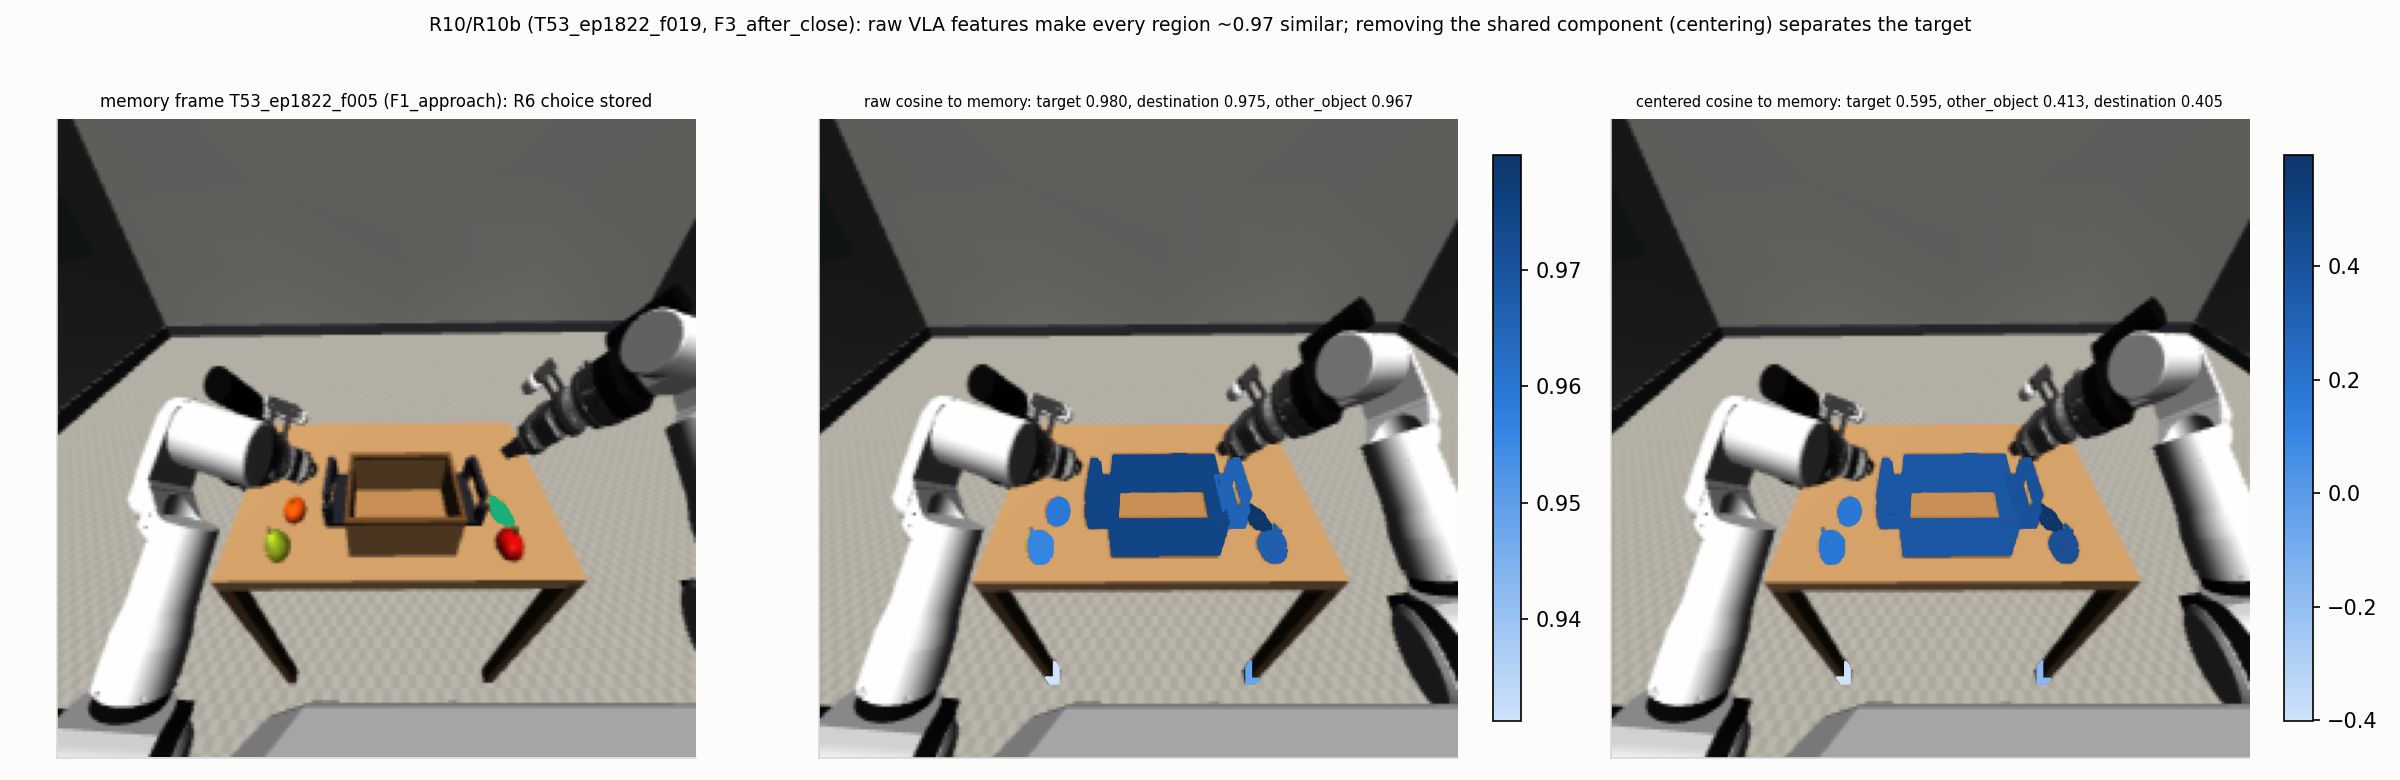
\includegraphics[width=\textwidth,height=.70\textheight,keepaspectratio]{../figures/ifg_results/exp/exp-R10-centering.png}
\caption{\textbf{R10/R10b: feature centering.} Can a stored descriptor distinguish alternative identities? The example is a base-grounding failure with a target region among the candidates. Raw target and destination cosine scores are 0.980 and 0.975; centered target and strongest-alternative scores are 0.595 and 0.413. Scales differ between panels. Descriptor separation in this example does not prove reliable region switching.}
\label{fig:supp-exp-R10-centering}
\end{figure*}

\begin{figure*}[p]
\centering
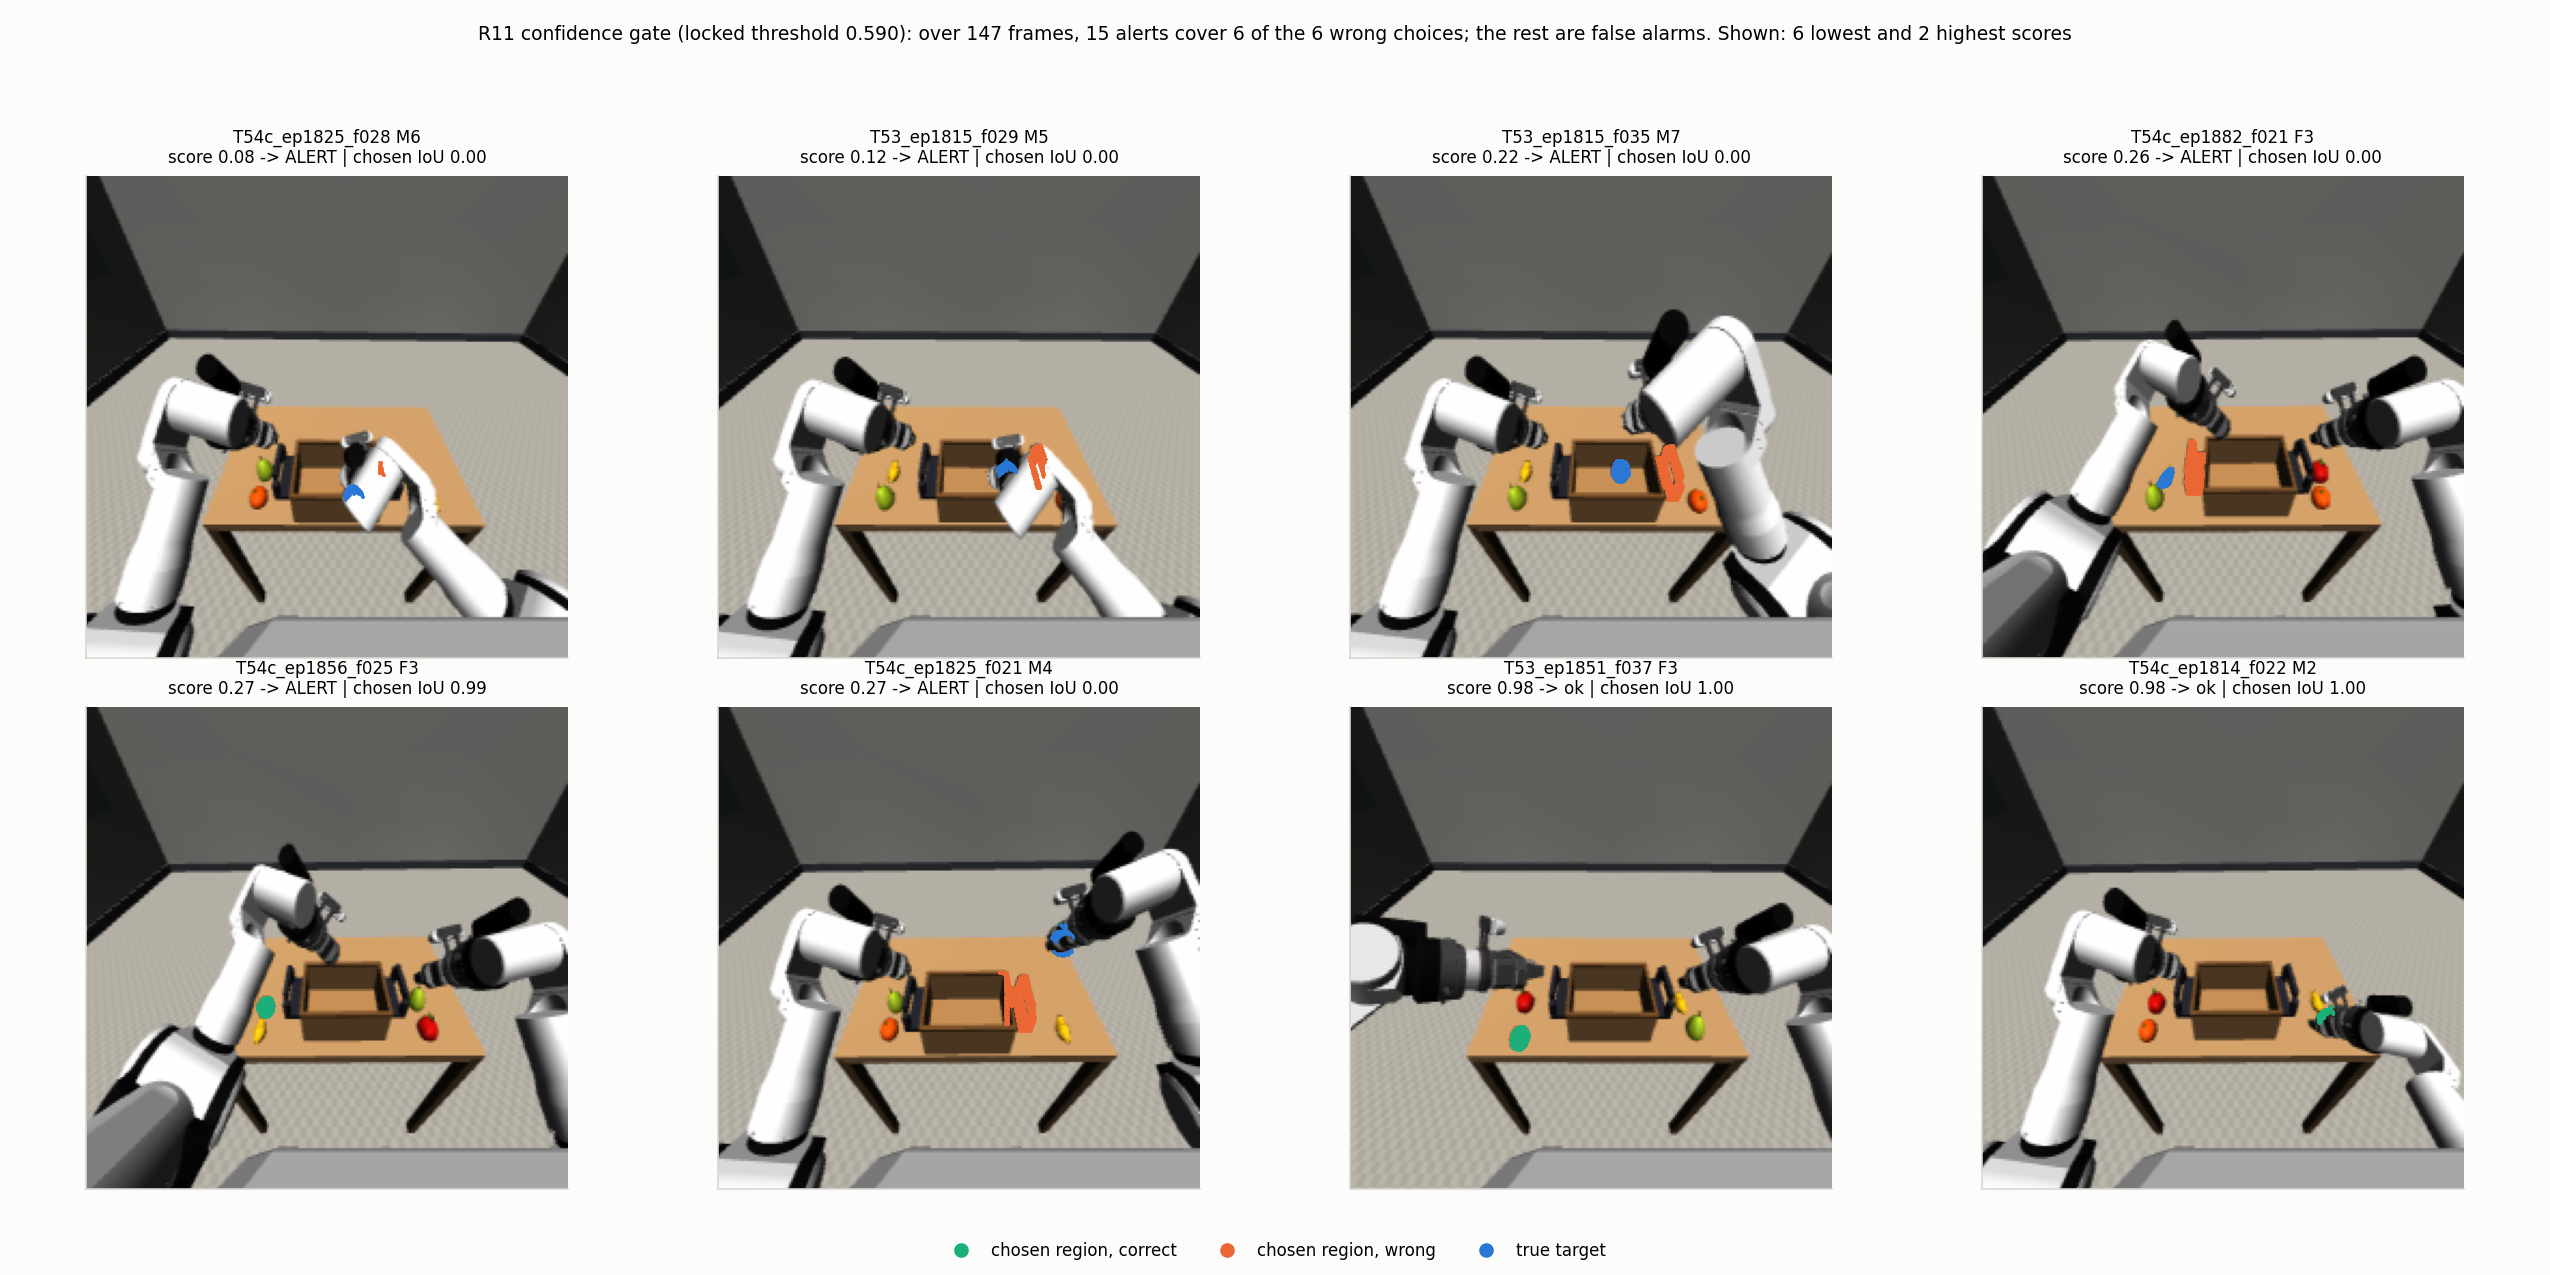
\includegraphics[width=\textwidth,height=.70\textheight,keepaspectratio]{../figures/ifg_results/exp/exp-R11-confidence-gate.png}
\caption{\textbf{R11: correct alerts and false alarms.} Does low temporal agreement flag a wrong choice? The gallery shows the six lowest and two highest centered chain scores, not all six errors. Across the 147-frame cohort, 15 alerts contain six wrong choices and nine other frames; the latter are false alarms under the IoU-below-0.1 definition. Emptying these predictions removes 81.6\% of false-positive mass and loses 6.0\% of true-positive mass. No controller or permission builder is run.}
\label{fig:supp-exp-R11-confidence-gate}
\end{figure*}

\begin{figure*}[p]
\centering
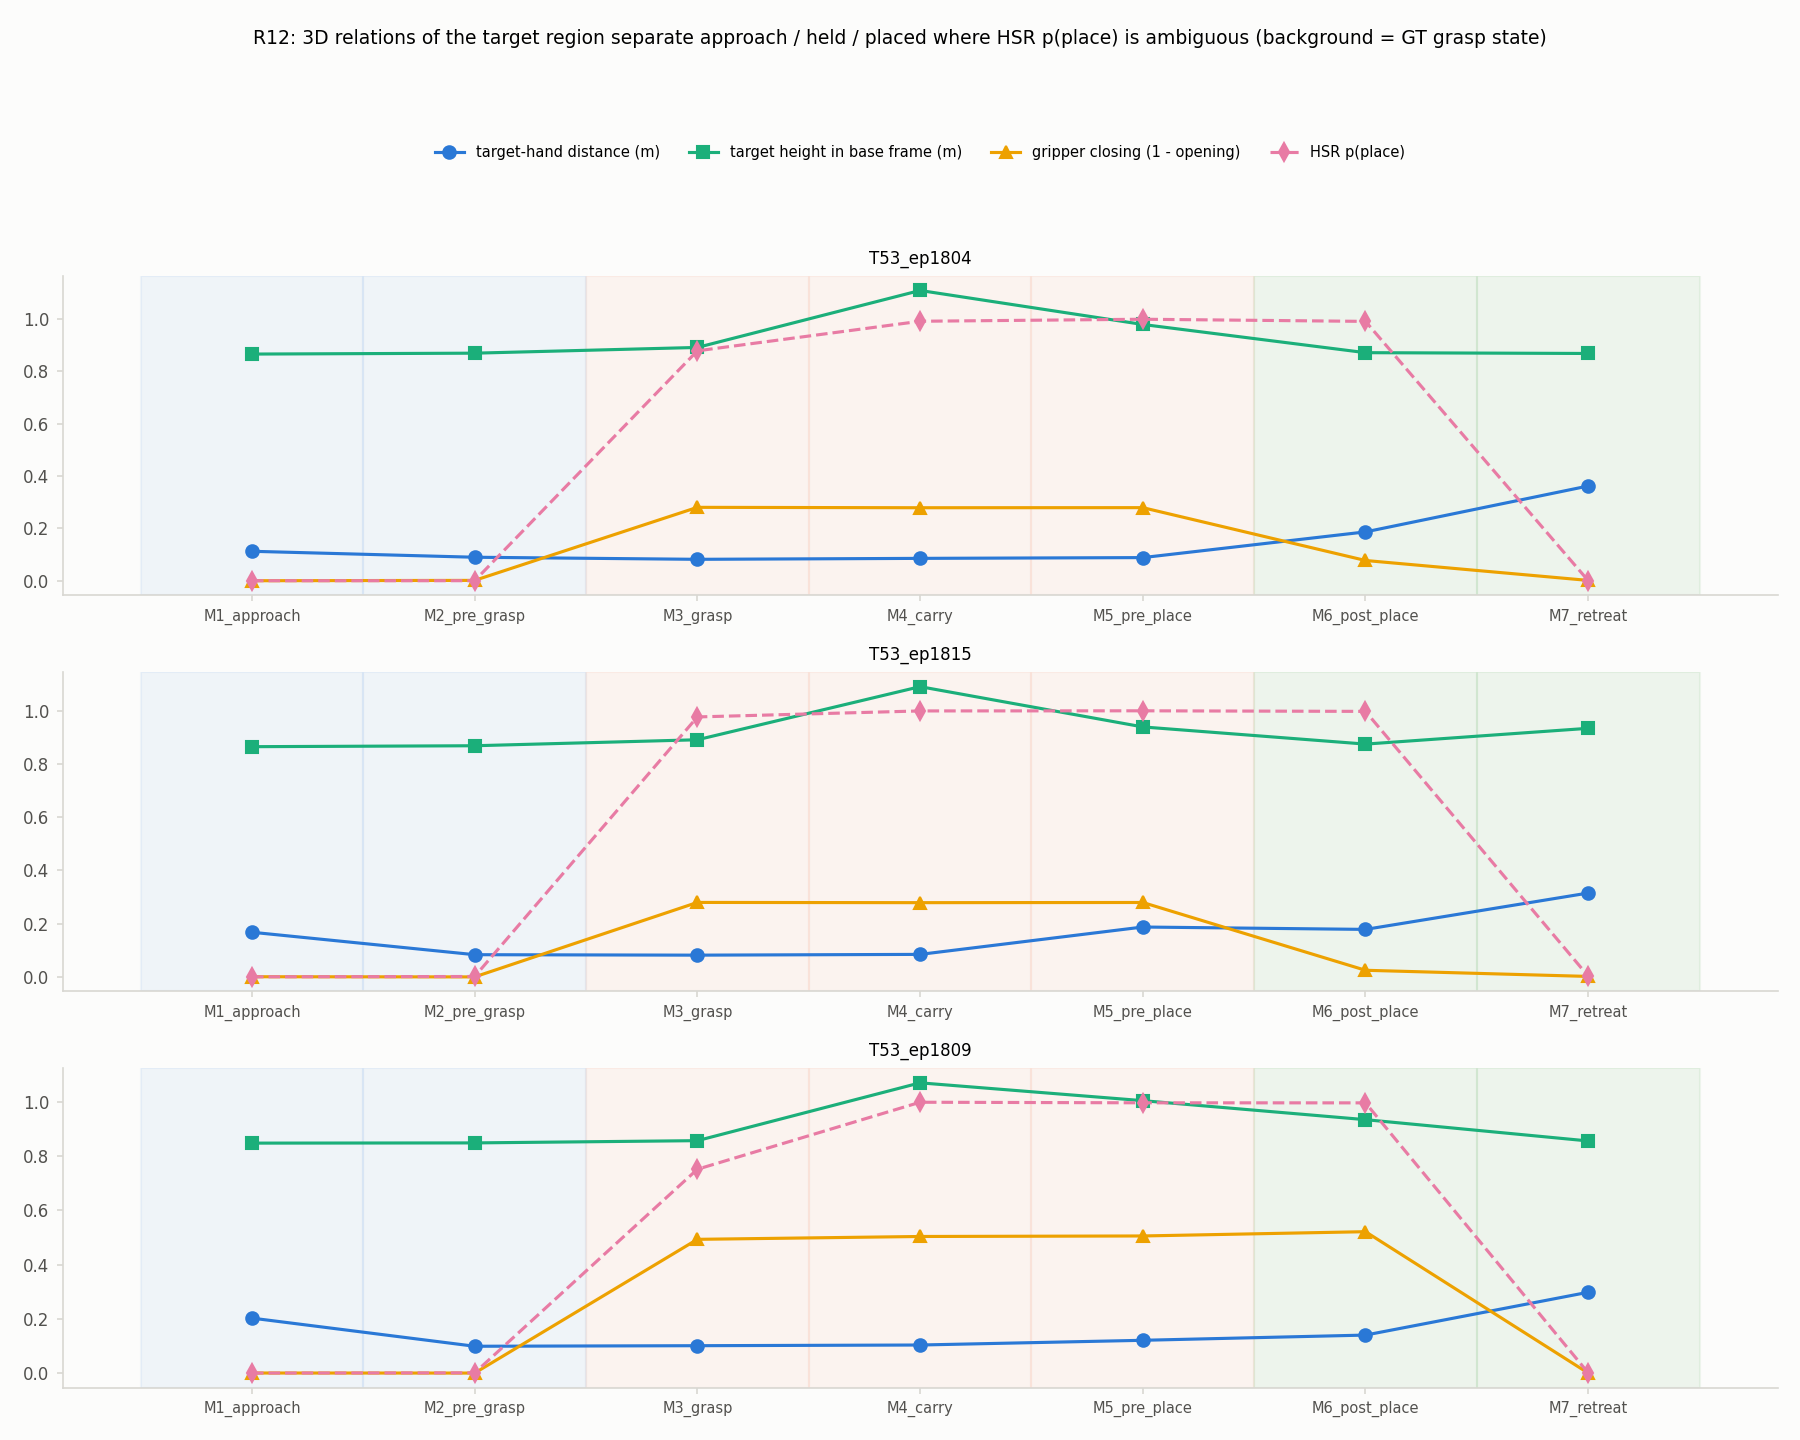
\includegraphics[width=\textwidth,height=.70\textheight,keepaspectratio]{../figures/ifg_results/exp/exp-R12-phase-3d.png}
\caption{\textbf{R12: geometry across task stages.} What state signals accompany approach, carrying, and retreat? These are the first three successful seven-frame episodes selected by the figure generator. Height is effectively floor-referenced, not clearance above the table. The adopted HSR-plus-gripper-plus-geometry classifier has pooled phase accuracy 0.939 and held-state accuracy 0.933 in leave-one-episode-out fitting; upstream development choices remain shared across folds.}
\label{fig:supp-exp-R12-phase-3d}
\end{figure*}

\clearpage
\end{document}
